\section{Knæartrosepatienter} \label{patientforlob}
\textit{Følgende afsnit omhandler knæleddet, knæartrose og patientgruppen. Afsnittet redegør for patientgruppen samt de forskellige disponeringsfaktorer for lidelsen. Dette vil danne grundlag for at klassificere gruppen af patienter, som tilbydes en TKA-operation. }

\subsection{Knæleddet og knæartrose}
Knæleddet er et synovialt, sammensat led med en bevægelsesgrad fra 0 til 135$\degree$ for fleksion og 0 til 5$\degree$ for hyperekstension. Knæleddet er kroppens største led, og er således udsat for større mekaniske påvirkninger end noget andet led i kroppen. Hermed oplever knæleddet hyppigere end noget andet led patologiske forandringer. Knæleddet er sammensat af tre knogler; femur, tibia og patella. Disse er alle på slidfladerne beklædt med et tykt lag hyalinbrusk. Dette lag kan være op til syv millimeter tykt. Sammen med meniskerne, der fordeler trykket på en større overflade, er hyalinbrusken med til at mindske friktionen i leddet. \citep{Moeller2001}

Knæartrose opdeles i en primær og sekundær tilstand. Den primære artrose betegner artrose, der opstår som følge af ikke-udefrakommende årsager, herunder genetik og aldring. Den sekundære artrose forårsages af tidligere skader, inflammation, overvægt og traume. Knæartrose er en tilstand, hvis hyppigste symptomer er smerter, nedsat mobilitet samt fejlstilling af leddet hos den påvirkede. Smerterne forekommer i forskellig grad fra igangsættende smerte til konstant smerte. Symptomerne forværres som lidelsen udvikler sig. \citep{Lind2016b}

\begin{figure}[H] 
	\begin{center}
		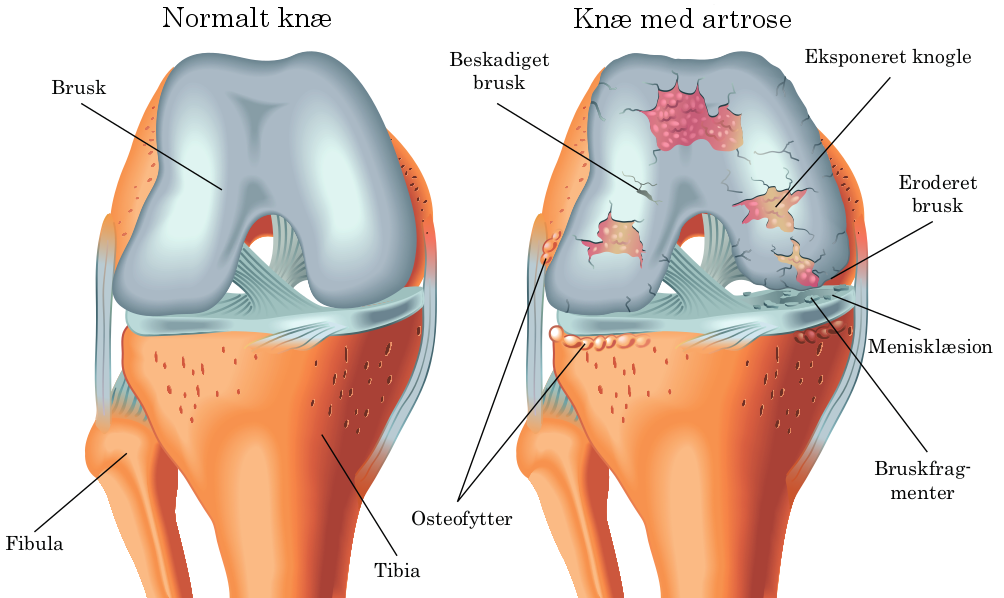
\includegraphics[width=0.6\textwidth]{figures/bProblemanalyse/Artose_knaePNG}
	\end{center}
	\caption{Figuren viser, hvad der sker i knæleddet, når det undergår patologiske forandringer ved knæartrose. Det ses af figuren til højre, at strukturne i knæet forandrer sig. Det fremgår, at bruskelementerne, ved infektion, slid eller traume, kan blive beskadiget, hvilket vil eksponere knoglen og føre til smerte og funktionsnedsættelse. På figuren til højre ses ligeledes osteofytter. \citep{schroder} \citep{adobe}} 
	\label{fig:tka_implant} 
\end{figure}

\textbf{inddrag figur. se note}

\subsection{Demografi}
En længere række faktorer har betydning for udviklingen af artrose. Hvis en eller flere af disse faktorer er til stede, er den påvirkede mere disponeret for knæartrose. Disse faktorer kan være alder, overbelastning ved arbejde og fritid, tidligere knæskader, genetisk arv, overvægt samt køn \citep{brostrom2012}. Knæartrose er til stede blandt 45~\% af alle 80-årige i befolkningen. Prævalensen for knæartose kan formodes at stige da levealderen i Danmark stiger. \\
En af risikofaktorerne for udviklingen af knæartrose er overvægt, hvilket 47~\% af den danske befolkning kan kategoriseres som \citep{Vestergaard2016}. Ydermere stiger andelen af overvægtige med alderen, hvilket ligeledes er tilfældet for knæartrose. Overvægtige med en høj body-mass-index (BMI>30 \citep{definitionfedme1999}) er disponeret for knæartrose med en relativ risiko på en faktor tre, hvoraf en kombination af ovenstående faktorer øger risikoen for lidelsen. Dog kan der opstå problematikker vedrørende benyttelsen af BMI, da metoden ikke skelner mellem fedt og muskler. \citep{brostrom2012} \citep{Lind2016b}




%Det kan antages, at der blandt nogle knæartrosepatienter findes en forventningsfaktor, der medfører, at de postoperativt kategoriserer sig selv som værende utilfredse, omend de har opnået en forbedring af både smerte, mobilitet eller begge. Denne antagelse understøttes af \citer{Bourne2010}, som beskriver de største prædiktorer for utilfredshed efter en TKA-operation. Den største faktor var, at patientens forventninger til operationen ikke blev mødt, hvilket medførte 10,7 gange større risiko for utilfredshed. \citep{Bourne2010} I et andet studie af \citer{Keudell2013} blev patienternes alder sammenkoblet med deres forventninger. Det tyder på, at patienter over 65 år har lavere forventninger til operationsresultatet end patienter under 65 år. De ældre patienter har ligeledes større tilfredshed end de yngre.\citep{Bourne2010} Dette kan antages at hænge sammen med et øget aktivitetsbehov hos yngre patienter. \textbf{Problem med kilder her!}

%Dette kan antages at have en sammenhæng med påstanden fra \cite{Bourne2010}, vedrørende prædiktoren til utilfredshed, omhandlende forventninger til operationen. \textbf{NOTE:(7 (mangler analyse?))}

%Utilfredshed hos patienterne kan være forårsaget af andre faktorer end kroniske postoperative smerter, herunder funktionsnedsættelse \citep{Jacobs2014}. 

%De præoperative tests indikerede, at der ikke var signifikant præoperativ forskel mellem patienterne for smerte eller funktion, blandt patienter som postoperative var tilfredse eller utilfredse. Postoperativt blev samme test udført og her var der signifikant forskel ved alle indikationer; passiv fleksion, smerte og funktion. 
%De patienter som var utilfredse efter operationen, havde signifikant dårligere resultater i forhold til passiv flektion, smerte og funktion, hvormed dette kan antages som værende grunden til patienternes utilfredshed. \citep{Jacobs2014} 

%I 2012 viste en undersøgelse fra Sundhedsstyrelsen, at 81 til 85\% af patienter, der havde modtaget en primær TKA-operation, var tilfredse, 8 til 11\% var decideret utilfredse og resten var i tvivl eller til dels utilfredse. Resultatet heraf er, at op mod 19\% af patienterne ikke opnår bedring fra deres smerter og eventuel nedsat mobilitet. \citep{brostrom2012} 
%Sundhedsstyrelsens indikationer vedrørende patientutilfredshed understøttes af flere internationale studier. Eksempelvis fandt studiet af \citer{Bourne2010}, at 19\% af de undersøgte patienter var utilfredse med resultatet af deres TKA-operation. Ydermere viser undersøgelser på tværs af tilsvarende studier, at andelen af utilfredse patienter befandt sig i området 11 til 25\%. \citep{Bourne2010} Et studie af \citer{Jacobs2014} undersøgte, om der er nogle bestemte karakteristika for patienter, som er utilfredse efter deres TKA-operation. \citer{Jacobs2014} fandt, at hverken alder, køn eller BMI havde en signifikant sammenhæng med om patienten var tilfreds eller utilfreds. 
%\begin{table}[H]
%	\centering
%\begin{tabular}{ccc}
%	\hline
%	\rowcolor[HTML]{C0C0C0} 
%	Studie            & Forsøgspopulation {[}N{]} & Utilfreds {[}\%{]} \\ \hline
%	Anderson et al.   & 74                        & 11                 \\
%	Noble et al.      & 253                       & 25                 \\
%	Robertsson et al. & 27.372                    & 18                 \\
%	Wylde et al.      & 228                       & 15                 \\
%	Hawker et al.     & 1193                      & 15                 \\
%	Heck et al.       & 291                       & 12                 \\
%	Bourne et al.     & 1703                      & 19                 \\
%	Petersen et al.	  & 215						  & 11				   \\ \hline
%\end{tabular}
%	\caption{I tabellen ses \cite{Bourne2010} sammenligning af flere studiers resultater vedrørende patientutilfredshed efterfulgt en primær TKA-operation. \citep{Bourne2010}\citep{Petersen2015}}
%	\label{tab:patient_utilfreds}
%\end{table}